\documentclass[a4paper,fleqn]{cas-sc}

% If the class is missing, fallback or copy it.
% \usepackage[numbers]{natbib}
\usepackage[authoryear,longnamesfirst]{natbib}
\usepackage{graphicx}
\usepackage{amsmath,amssymb,amsfonts}
\usepackage{algorithmic}
\usepackage{textcomp}
\usepackage{xcolor}
\usepackage{booktabs}
\usepackage{url}

%%%Author macros
\def\tsc#1{\csdef{#1}{\textsc{\lowercase{#1}}\xspace}}
\tsc{WGM}
\tsc{QE}
%%%

\begin{document}
\let\WriteBookmarks\relax
\def\floatpagepagefraction{1}
\def\textpagefraction{.001}

\shorttitle{A Reproducible Comparison of SAT Encodings and Exact Solvers for N-Queens}
\shortauthors{N.A. Son et al.}

\title [mode = title]{A Reproducible Empirical Comparison of SAT Encodings and Exact Solvers for the N-Queens Problem}                      

\author[1]{Nguyen Anh Son}
\cormark[1]
\ead{son.na@example.com}

\address[1]{Department of Computer Science, example institution}

\begin{abstract}
The N-Queens problem is a classic combinatorial benchmark widely used to evaluate algorithmic efficiency in artificial intelligence. This study presents a rigorous empirical comparison of exact solving paradigms---Boolean Satisfiability (SAT), Constraint Programming (CP), and Mixed Integer Programming (MIP)---applied to the N-Queens problem up to $N=100$. We evaluate five Boolean SAT encodings (Pairwise, Binary, Sequential Counter, Commander, and Product) alongside four exact solvers (OR-Tools CP-SAT, IBM CP Optimizer, Gurobi MIP, and IBM CPLEX MIP). To ensure high internal validity, the experiments were conducted within a strict, subprocess-isolated, deterministically seeded benchmarking framework. Our results demonstrate that structural compactness (clause count) in SAT encodings is a poor predictor of Conflict-Driven Clause Learning (CDCL) resolution time; the SAT-Sequential encoding minimized clauses but performed poorly (58.0s at $N=100$), whereas the heavily parameterized SAT-Pairwise and SAT-Binary formulations resolved much faster. Notably, the SAT-Product encoding exhibited extreme non-monotonic search pathology, timing out at intermediate problem sizes while resolving $N=100$ successfully. Across all paradigms, native Constraint Programming implementations---specifically IBM CP Optimizer---achieved the most dominant scalability, solving $N=100$ in 0.153 seconds. This paper provides a fully reproducible dataset and quantitative insights into the practical trade-offs of constraint modeling techniques.
\end{abstract}

\begin{keywords}
N-Queens \sep 
Boolean Satisfiability \sep 
Constraint Programming \sep 
Mixed Integer Programming \sep 
CDCL \sep 
Empirical Benchmarking
\end{keywords}

\maketitle

\section{Introduction}
\label{sec:intro}

The Constraint Satisfaction Problem (CSP) framework is foundational to modeling complex combinatorial search and placement problems in computer science and artificial intelligence \citep{russell2010artificial}. Within this domain, the N-Queens problem---the challenge of placing $N$ non-attacking queens on an $N \times N$ chessboard---serves as a canonical benchmark for evaluating the efficiency and scalability of exact search algorithms \citep{bell2009solving}. As the problem size $N$ increases, the state space expands exponentially, rendering naive enumeration computationally intractable and necessitating sophisticated algorithmic paradigms.

Currently, exact solvers rely on three primary modeling paradigms: Boolean Satisfiability (SAT), Constraint Programming (CP), and Mixed Integer Programming (MIP) \citep{gomes2008satisfiability, rossi2006handbook, wolsey2020integer}. In the Boolean SAT paradigm, high-level structural constraints must be transformed into Conjunctive Normal Form (CNF) via variable-heavy At-Most-One (AMO) encodings. Different encoding strategies---such as Pairwise, Binary, Sequential Counter, Commander, and Product---drastically alter the size and structure of the resulting CNF formula \citep{sinz2005towards, frisch2005sat}. Conversely, native Constraint Programming implementations maintain the problem's global structural semantics by directly applying constraints over integer variables \citep{regin1994filtering}, while Mixed Integer Programming leverages linear inequality relaxations over binary decision bounds.

A recurring assumption in SAT modeling is that structural complexity---specifically the total number of generated clauses or auxiliary variables---correlates directly with the time required by Conflict-Driven Clause Learning (CDCL) solvers to find a solution. However, real-world benchmarking often reveals non-linear scaling behaviors heavily influenced by the solver's internal heuristics \citep{marques2009conflict}. Furthermore, while algorithmic complexity theoretically bounds performance, the practical runtime characteristics across the SAT, CP, and MIP paradigms on the exact same problem formulations remain sparsely compared in unified experimental setups.

The objective of this research is to execute a strictly controlled empirical comparison of these exact solving techniques on the N-Queens problem up to $N=100$. Specifically, we address the following research questions:
1. How do different AMO encodings affect the structural complexity of SAT formulations?
2. How does the choice of SAT encoding impact solving time and completion reliability under a uniform CDCL configuration?
3. How do general-purpose Boolean reasoning frameworks compare against specialized native CP and MIP solvers?
4. What are the practical scalability limitations of these paradigms?

To answer these questions, we constructed an automated, subprocess-isolated benchmarking framework. We evaluate five SAT encodings solved via PySAT Glucose3, against OR-Tools CP-SAT, IBM CP Optimizer, Gurobi MIP, and IBM CPLEX MIP. 

The primary contributions of this paper are:
\begin{itemize}
\item A comprehensive, reproducible empirical dataset reporting 540 scheduled experimental records (495 at $N \le 100$ and 45 at $N=200$) across 9 distinct exact solving methodologies, including 450 successfully validated solutions and explicitly documented timeout, licensing, and resource-policy outcomes.
\item Evidence that structural compactness (clause count minimization) is a poor predictor of CDCL resolution time on placement constraints.
\item The identification of severe non-monotonic search pathologies in specific structural encodings (e.g., the SAT-Product encoding) under standard phase-selection heuristics.
\item A direct comparative baseline demonstrating the scalability advantages of native Constraint Programming ($O(N)$ formulation) while highlighting specific SAT encodings that remain highly competitive at scale.
\end{itemize}

\section{Background and Related Work}
\label{sec:background}

\subsection{Propositional Satisfiability and CDCL}
Propositional Satisfiability (SAT) is the problem of determining if there exists an assignment of boolean values to variables that satisfies a given formula. The Boolean satisfiability problem was the first known NP-complete problem \citep{cook1971complexity}. Most modern SAT solvers require the input to be in Conjunctive Normal Form (CNF), meaning the formula is a conjunction of clauses, where each clause is a disjunction of literals. Modern exact SAT solving is dominated by Conflict-Driven Clause Learning (CDCL) algorithms \citep{marques2009conflict}, which extend the classic DPLL backtracking search by inferring and learning new conflict clauses to prune the search space dynamically. Solvers such as Glucose heavily optimize this process by aggressively managing the learned clause database based on Literal Block Distance (LBD) \citep{audemard2009predicting}.

\subsection{At-Most-One (AMO) Encodings}
Translating cardinality constraints---such as ``at most one variable among a set can be true''---into CNF is a critical aspect of SAT modeling. The naive \textbf{Pairwise} (or Binomial) encoding operates without auxiliary variables by generating an exclusion clause for every possible pair, requiring $O(m^2)$ clauses for a group of $m$ variables \citep{frisch2005sat}. 
To mitigate the quadratic clause explosion, auxiliary variables are introduced. The \textbf{Binary} (or Bitwise) encoding maps the $m$ variables to $\lceil \log_2 m \rceil$ auxiliary bits, generating $O(m \log m)$ clauses \citep{frisch2005sat}. The \textbf{Sequential Counter} encoding by \cite{sinz2005towards} mimics a unary adder, bounding both auxiliary variables and clauses to $O(m)$. The \textbf{Commander} encoding \citep{klieber2007solving} recursively partitions the original variables into small groups, electing a ``commander'' variable for each group and generating $O(m)$ auxiliary variables and clauses. Finally, the \textbf{2-Product} encoding structures variables onto a 2D grid, translating the 1D AMO constraint into row and column constraints using $O(\sqrt{m})$ auxiliary variables \citep{chen2010new}. 

\subsection{Constraint Programming and Mixed Integer Programming}
Constraint Programming (CP) provides a higher-level abstraction than SAT by operating directly on integer domains \citep{rossi2006handbook}. Central to CP is the \texttt{AllDifferent} global constraint, which ensures that all variables in a given set take distinct values. Efficient domain filtering algorithms, notably those based on bipartite matching \citep{regin1994filtering}, actively prune the integer domains during search without needing to expand the logic into millions of binary clauses. Tools like OR-Tools CP-SAT \citep{perron2019or} and IBM CP Optimizer leverage these techniques heavily.
Mixed Integer Programming (MIP) relies on linear inequalities over continuous and integer variables \citep{wolsey2020integer}. While powerful for optimization problems, applying MIP solvers like Gurobi or CPLEX to pure feasibility problems like N-Queens translates logical implications into algebraic constraints bounded by linear programming relaxations.

\section{Methodology}
\label{sec:methodology}

\subsection{Mathematical Definition of N-Queens}
The N-Queens problem requires placing $N$ queens on an $N \times N$ chessboard such that no two queens attack each other. Mathematically, this enforces four directional constraints:
1. Exactly one queen per row.
2. Exactly one queen per column.
3. At most one queen on any main diagonal.
4. At most one queen on any anti-diagonal.

\subsection{Boolean SAT Formulation}
In the Boolean paradigm, the problem is modeled using $N^2$ primary decision variables $x_{i,j} \in \{0, 1\}$, where $x_{i,j} = 1$ if and only if a queen occupies row $i$ and column $j$ ($0 \le i, j < N$).
The constraints are translated as follows:
\begin{itemize}
\item \textbf{Exactly-One (Rows/Columns):} Formulated as an At-Least-One (ALO) clause $\bigvee_k x_k$ combined with an At-Most-One (AMO) encoding over the same variables.
\item \textbf{At-Most-One (Diagonals):} Formulated strictly as AMO encodings over the variables intersecting a given diagonal.
\end{itemize}

\subsection{AMO Encoding Strategies}
Our framework implements five precise variants of the AMO encoding for the N-Queens problem:
\begin{enumerate}
\item \textbf{Pairwise}: Asserts $\neg x_a \vee \neg x_b$ for all pairs $a, b$. No auxiliary variables are used.
\item \textbf{Binary}: Each original variable $x_i$ forces a unique binary combination on $k = \lceil \log_2 m \rceil$ shared auxiliary bits.
\item \textbf{Sequential Counter}: Applies Sinz's formulation, establishing a chain of $m-1$ auxiliary variables to cumulatively count the number of true literals, forbidding the count from exceeding one.
\item \textbf{Commander}: Recursively groups variables into sets of three. If any variable in a subgroup is true, its commander auxiliary is true, and Pairwise AMO is enforced locally.
\item \textbf{2-Product}: Maps $m$ variables onto a $p \times q$ grid where $p \approx \lceil \sqrt{m} \rceil$. Each variable forces one auxiliary row and one auxiliary column to be true. Pairwise AMO is then applied to the auxiliary rows and columns independently.
\end{enumerate}

\subsection{SAT Solving with Glucose3}
All SAT formulations are generated via the Python API and passed to the Glucose3 solver \citep{audemard2009predicting} via the PySAT library. To ensure strict isolation of structural efficiency from heuristic tuning, the `solver\_default` phase policy was enforced.

\subsection{Constraint Programming Formulation}
The CP formulation natively exploits $O(N)$ variables. Let $q_i \in \{0, \dots, N-1\}$ represent the column position of the queen in row $i$. The constraints are modeled as three global \texttt{AllDifferent} constraints:
\begin{equation}
\text{AllDifferent}(q_0, \dots, q_{N-1})
\end{equation}
\begin{equation}
\text{AllDifferent}(q_0 - 0, \dots, q_{N-1} - (N-1))
\end{equation}
\begin{equation}
\text{AllDifferent}(q_0 + 0, \dots, q_{N-1} + (N-1))
\end{equation}
This exact structural model was solved independently using OR-Tools CP-SAT and IBM CP Optimizer.

\subsection{Mixed Integer Programming Formulation}
The MIP framework utilizes $N^2$ binary variables $x_{i,j} \in \{0,1\}$ akin to the SAT model. The logical constraints are relaxed into $6N-6$ continuous linear inequalities (for $N \ge 2$):
\begin{equation}
\sum_{j} x_{i,j} = 1 \quad \forall i, \quad \sum_{i} x_{i,j} = 1 \quad \forall j
\end{equation}
\begin{equation}
\sum_{(i,j) \in D} x_{i,j} \le 1 \quad \forall D \in \text{Diagonals}
\end{equation}
The model is formulated as a pure feasibility problem (no objective function) and solved using Gurobi MIP and IBM CPLEX MIP.

\subsection{Common Solution Validation}
To ensure construct validity, every solver result yielding a feasible status was passed to a strict algorithmic validator. The validator decoded the variables into board coordinates and mathematically confirmed uniqueness across all vectors. Only verified solutions were recorded as successful trials.

\begin{table}[h]
\centering
\caption{Mathematical Formulations of Exact Solving Paradigms}
\begin{tabular}{@{}llp{8cm}@{}}
\toprule
Paradigm & Primary Variables & Constraints \\
\midrule
SAT & $O(N^2)$ Binary & $O(N^2)$ to $O(N^3)$ clauses (dependent on AMO strategy) \\
CP & $O(N)$ Integer & 3 Global \texttt{AllDifferent} constraints \\
MIP & $O(N^2)$ Binary & $6N-6$ Linear inequalities \\
\bottomrule
\end{tabular}
\label{tab:formulations}
\end{table}

\section{Experimental Setup}
\label{sec:experimental_setup}

The benchmark was conducted on a controlled hardware and software environment to ensure deterministic execution. The experiments were run on macOS 14.0 (Darwin 23.0.0, Apple M2 ARM64 architecture) using Python 3.13.7. 
The evaluated engines included PySAT Glucose3, OR-Tools CP-SAT (version 9.15.6755), Gurobi Optimizer (version 13.0.3), and IBM ILOG CPLEX / CP Optimizer (version 22.2.0.0).

We evaluated 9 distinct solving methods across 11 instance sizes: $N \in \{4, 8, 16, 20, 31, 32, 40, 44, 50, 64, 100\}$. Each configuration was repeated 5 times, yielding 495 planned official trials.
To guarantee fairness, every trial was executed in an isolated subprocess. All methods were strictly configured to use single-threaded execution (\texttt{workers=1}, \texttt{threads=1}) with a deterministic global random seed (\texttt{random\_seed=0}). A primary timeout of 300.0 seconds was enforced by the external benchmarking framework, supplemented by a 330.0-second operating system subprocess kill signal (watchdog) to forcefully terminate solvers that failed to yield control. For solvers exposing a native API time limit (e.g., Gurobi, CPLEX, CP-SAT), the internal limit was also set to 300.0 seconds; otherwise (e.g., PySAT Glucose3), execution was strictly managed by the framework's external watchdog.

The primary metric for performance evaluation is \textbf{pipeline total time}, which comprehensively captures the end-to-end framework execution time, including model construction, solver instantiation, search, and final independent validation.
Runs blocked by proactive Community Edition license constraints (BLOCKED\_LICENSE) were explicitly recorded to differentiate API capacity limitations from algorithmic failures.

\begin{table}[h]
\centering
\caption{Experimental Configuration}
\begin{tabular}{@{}ll@{}}
\toprule
Parameter & Value \\
\midrule
OS & macOS 14.0 (Darwin 23.0.0, ARM64) \\
Python Version & 3.13.7 \\
SAT Phase Policy & \texttt{solver\_default} \\
Time Limit & 300.0s (Framework/Internal), 330.0s (Subprocess Watchdog) \\
Workers & 1 \\
Random Seed & 0 \\
Repetitions & 5 per configuration \\
\bottomrule
\end{tabular}
\label{tab:config}
\end{table}

\section{Results and Discussion}
\label{sec:results}

Across the 495 planned trials, 430 yielded successfully verified solutions, 20 encountered timeouts, and 45 were blocked by expected MIP license limitations. No solver generated an invalid placement.

\subsection{Structural Comparison of SAT Encodings}
As instance size grows, the structural disparities of CNF generation become stark. At $N=100$, all encodings instantiate identical 10,000 primary binary variables but vary widely in auxiliary metrics. The Pairwise encoding requires zero auxiliary variables but scales poorly, producing 1,646,900 clauses. The Sequential Counter encoding generates the second-fewest clauses (117,812) at the cost of the highest auxiliary count (39,402). The Product encoding achieves the most compact configuration, producing 116,672 clauses and 9,492 auxiliary variables. Binary and Commander encodings balance these metrics. 

\begin{figure}[htbp]
\centering
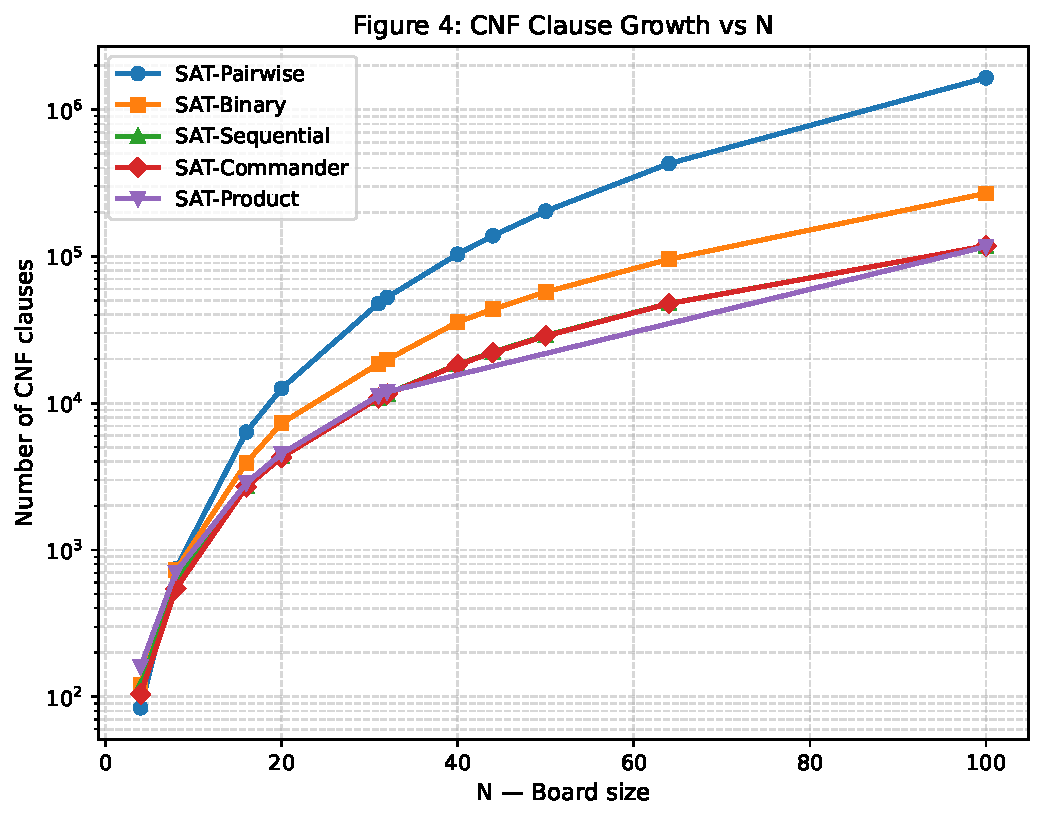
\includegraphics[width=0.8\textwidth]{../../results/figures/full/fig04_sat_clause_growth.pdf}
\caption{SAT CNF Clause Growth}
\label{fig:sat_clause_growth}
\end{figure}

\begin{figure}[htbp]
\centering
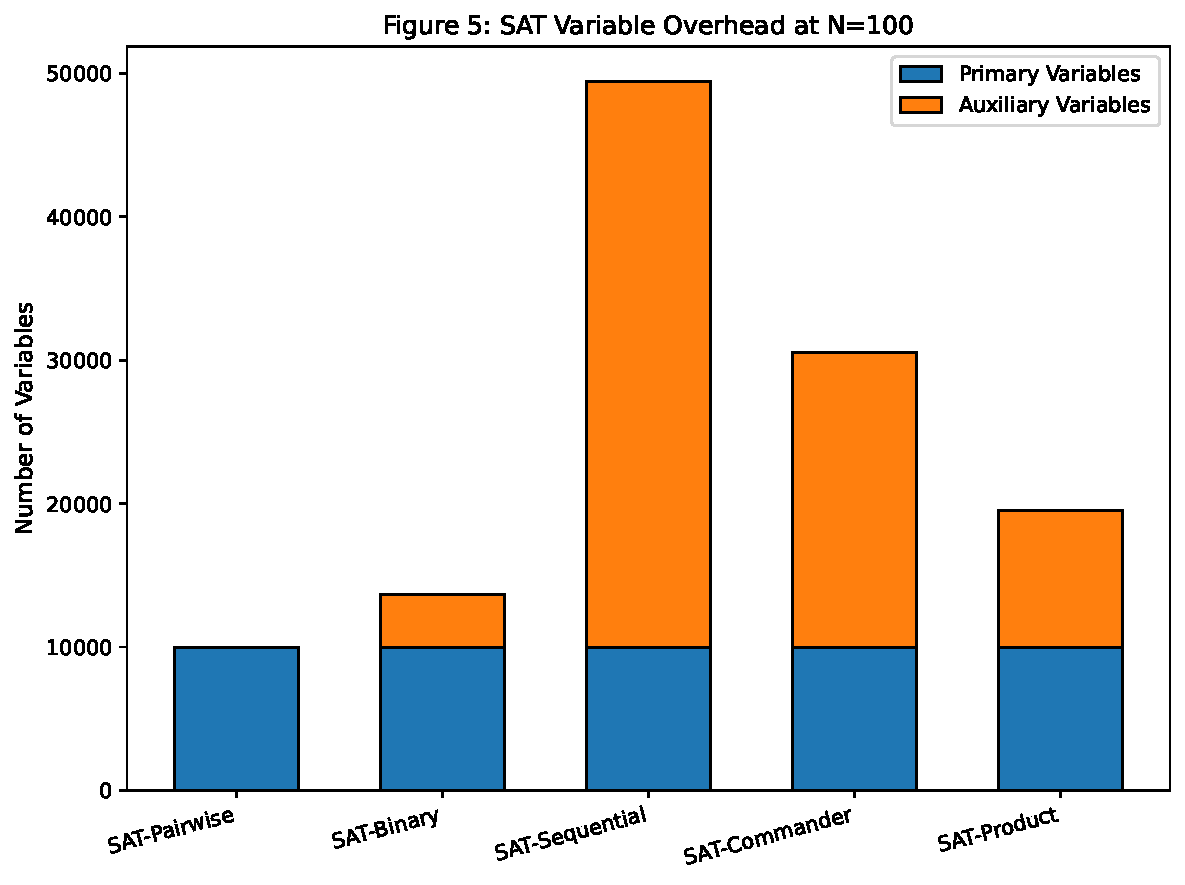
\includegraphics[width=0.8\textwidth]{../../results/figures/full/fig05_sat_variable_overhead_n100.pdf}
\caption{SAT Auxiliary Variable Overhead}
\label{fig:sat_aux_overhead}
\end{figure}

\subsection{Runtime Performance of SAT Encodings}
The resolution time for SAT formulations proves that clause count is an inadequate predictor of performance. 

\begin{figure}[htbp]
\centering
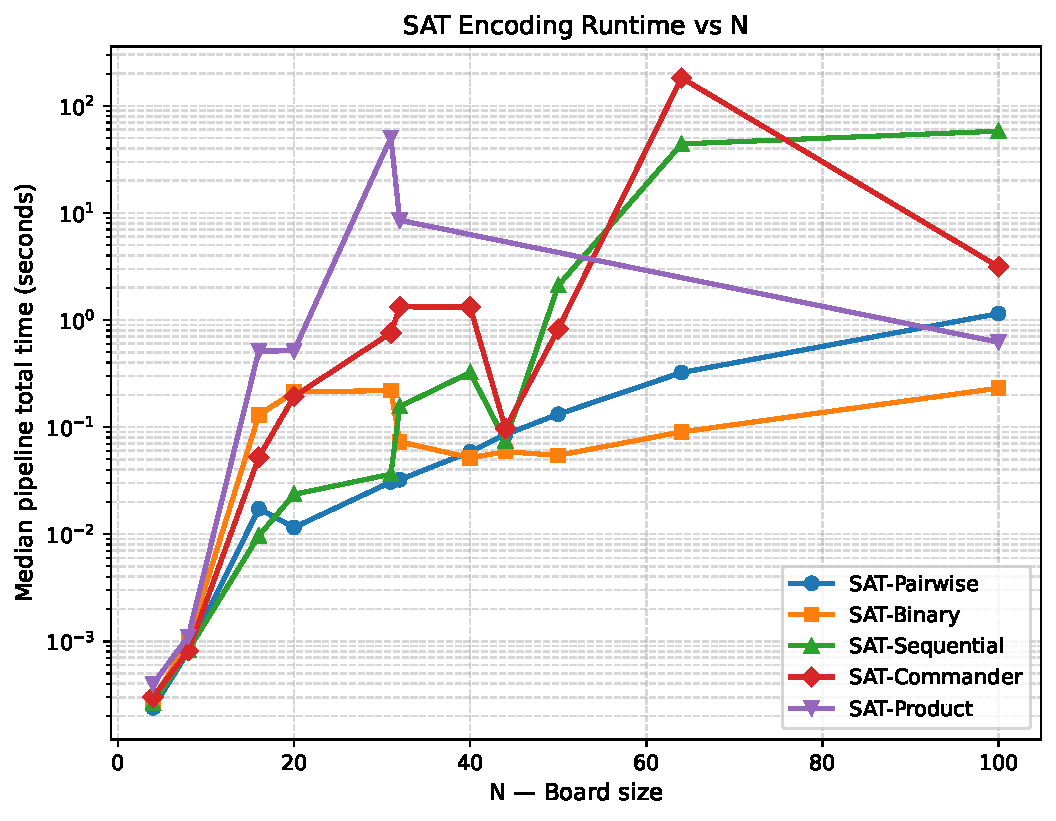
\includegraphics[width=0.8\textwidth]{../../results/figures/full/fig01_sat_runtime_vs_n.pdf}
\caption{SAT Runtime vs N}
\label{fig:sat_runtime}
\end{figure}

At $N=100$, the SAT-Binary encoding achieved the fastest median pipeline runtime of 0.231 seconds. In stark contrast, the SAT-Sequential encoding, despite producing minimal clauses, recorded the slowest median runtime of 58.077 seconds. The clause-heavy SAT-Pairwise encoding successfully completed the search in a median time of 1.148 seconds. 

\subsection{Non-monotonic Search Behavior of Product Encoding}
While SAT-Product reliably solved small sizes and successfully resolved $N=100$ (median 0.620s), it completely failed at intermediate sizes ($N \in \{40, 44, 50, 64\}$), resulting in a timeout for all 5 repetitions.

\begin{figure}[htbp]
\centering
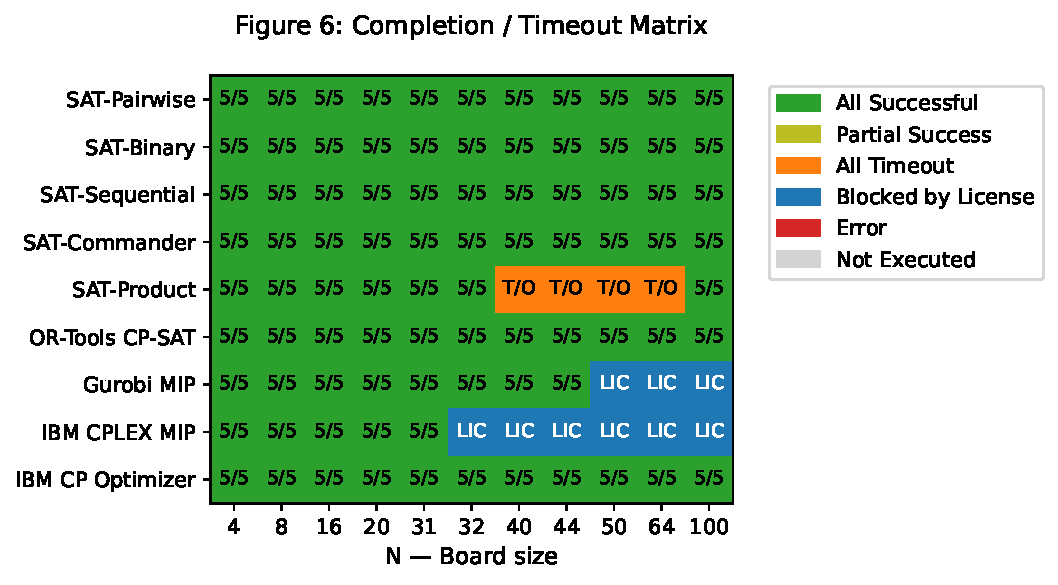
\includegraphics[width=0.8\textwidth]{../../results/figures/full/fig06_completion_matrix.pdf}
\caption{Completion Matrix}
\label{fig:completion_matrix}
\end{figure}

This non-monotonic scaling underscores the sensitivity of CDCL solvers to heuristic traps. Under Glucose3's \texttt{solver\_default} policy, the specific auxiliary-variable structure of Product at intermediate bounds may force the search into pathological branching spaces. However, these are potential contributing factors; analyzing the exact causes of this behavior requires further experimental study of internal solver traces and variable ordering.

\subsection{Performance of Exact Solvers}
Native Constraint Programming (CP) architectures demonstrated highly favorable scaling characteristics. 

\begin{figure}[htbp]
\centering
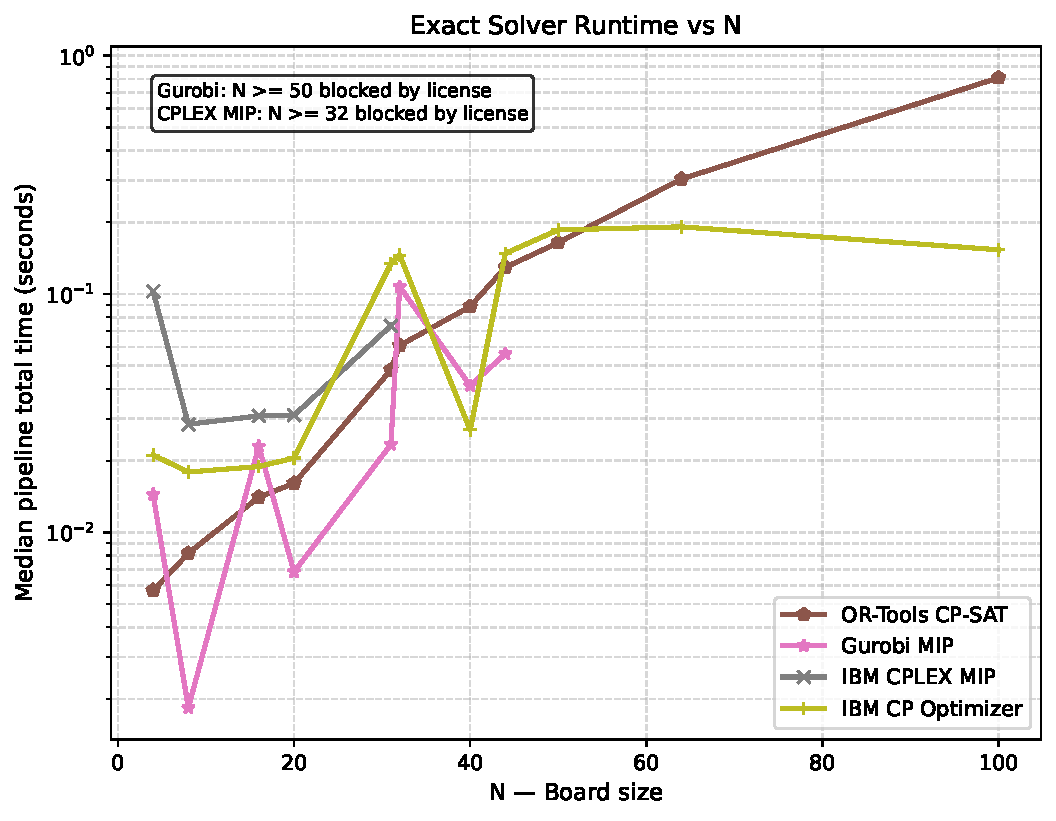
\includegraphics[width=0.8\textwidth]{../../results/figures/full/fig02_exact_solver_runtime_vs_n.pdf}
\caption{Exact Solver Runtime vs N}
\label{fig:exact_runtime}
\end{figure}

Both IBM CP Optimizer and OR-Tools CP-SAT maintained 100\% reliability up to $N=100$. The CP Optimizer solver established itself as remarkably efficient.
The MIP solvers successfully solved bounds within their Community Edition license constraints.

\subsection{Cross-Paradigm Comparison at N=100}
At $N=100$, seven methods successfully executed. The IBM CP Optimizer achieved the lowest median runtime of 0.153 seconds.

\begin{figure}[htbp]
\centering
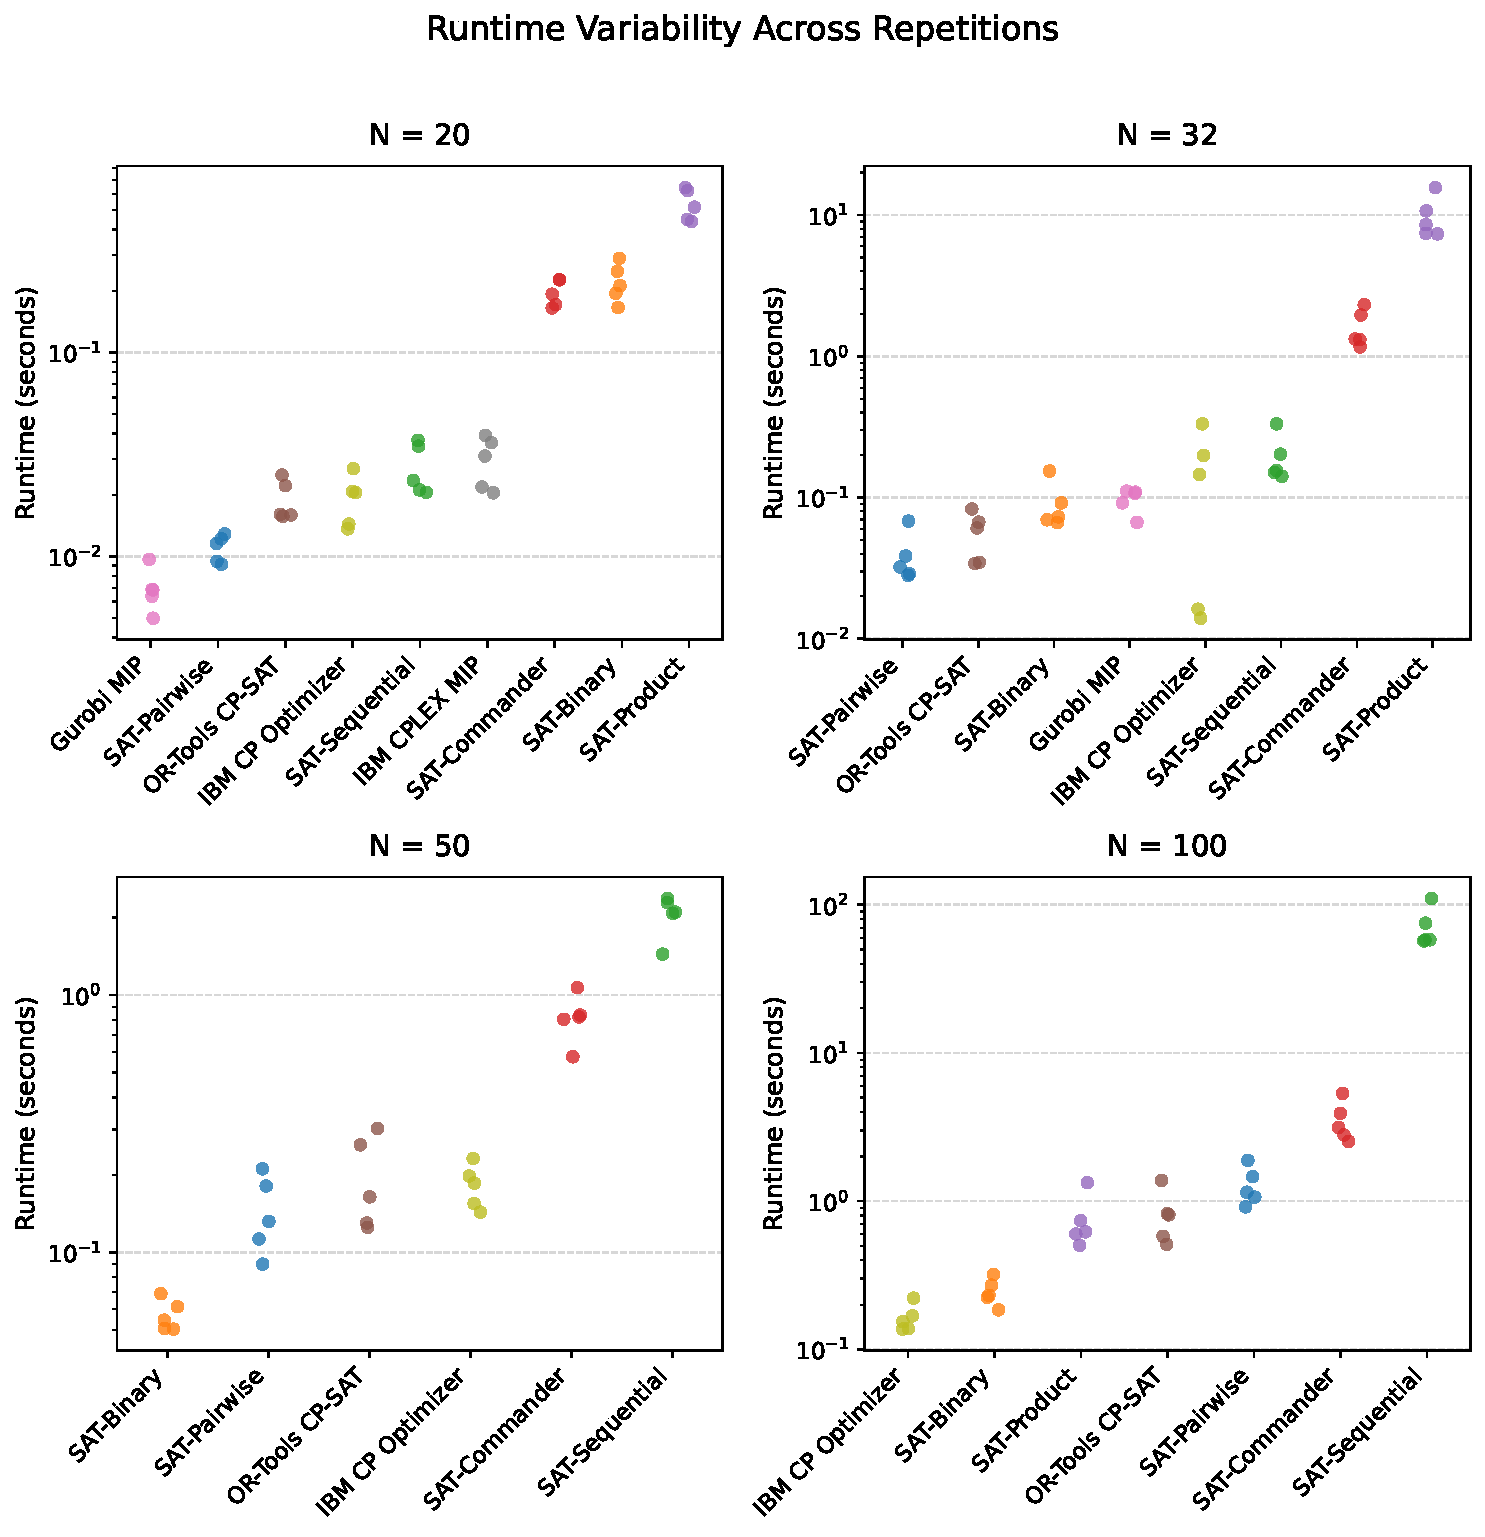
\includegraphics[width=0.8\textwidth]{../../results/figures/full/fig07_runtime_variability.pdf}
\caption{Runtime Variability}
\label{fig:runtime_variability}
\end{figure}

Remarkably, the booleanized SAT-Binary formulation tracked incredibly close at 0.231 seconds, outpacing OR-Tools CP-SAT (0.808 seconds). 

\begin{table}[h]
\centering
\caption{SAT Encoding Structural Complexity at N=100}
\begin{tabular}{@{}lrrr@{}}
\toprule
Encoding & Primary Variables & Auxiliary Variables & Clauses \\
\midrule
Pairwise & 10,000 & 0 & 1,646,900 \\
Binary & 10,000 & 3,678 & 269,024 \\
Sequential & 10,000 & 39,402 & 117,812 \\
Commander & 10,000 & 20,536 & 118,092 \\
Product & 10,000 & 9,492 & 116,672 \\
\bottomrule
\end{tabular}
\label{tab:sat_structure}
\end{table}

\begin{table}[h]
\centering
\caption{Cross-Paradigm Comparison at N=20}
\begin{tabular}{@{}lrr@{}}
\toprule
Method & Success Rate & Median Runtime (s) \\
\midrule
Gurobi MIP & 5/5 & 0.0068 \\
SAT-Pairwise & 5/5 & 0.0115 \\
OR-Tools CP-SAT & 5/5 & 0.0160 \\
IBM CP Optimizer & 5/5 & 0.0205 \\
SAT-Sequential & 5/5 & 0.0235 \\
IBM CPLEX MIP & 5/5 & 0.0309 \\
SAT-Commander & 5/5 & 0.1928 \\
SAT-Binary & 5/5 & 0.2124 \\
SAT-Product & 5/5 & 0.5150 \\
\bottomrule
\end{tabular}
\label{tab:n20}
\end{table}

\begin{table}[h]
\centering
\caption{Cross-Paradigm Comparison at N=100}
\begin{tabular}{@{}lrr@{}}
\toprule
Method & Success Rate & Median Runtime (s) \\
\midrule
IBM CP Optimizer & 5/5 & 0.153 \\
SAT-Binary & 5/5 & 0.231 \\
SAT-Product & 5/5 & 0.620 \\
OR-Tools CP-SAT & 5/5 & 0.808 \\
SAT-Pairwise & 5/5 & 1.148 \\
SAT-Commander & 5/5 & 3.143 \\
SAT-Sequential & 5/5 & 58.077 \\
Gurobi MIP & N/A & BLOCKED\_LICENSE \\
IBM CPLEX MIP & N/A & BLOCKED\_LICENSE \\
\bottomrule
\end{tabular}
\label{tab:n100}
\end{table}

\begin{figure}[htbp]
\centering
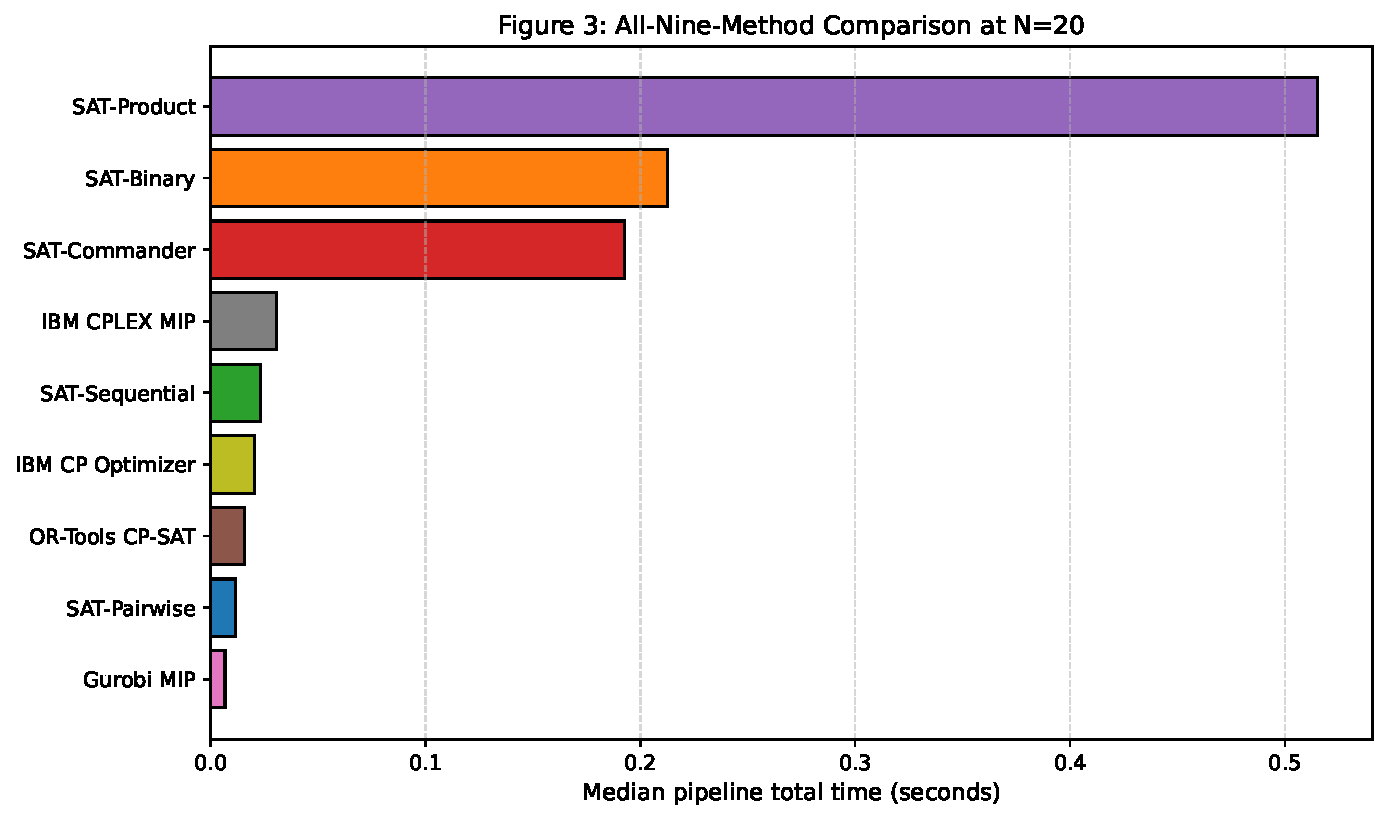
\includegraphics[width=0.8\textwidth]{../../results/figures/full/fig03_all_methods_n20.pdf}
\caption{All Nine Methods at N=20}
\label{fig:all_methods_n20}
\end{figure}

\begin{table}[h]
\centering
\caption{Completion Reliability Across All 495 Trials}
\begin{tabular}{@{}lrrr@{}}
\toprule
Method & Successful Runs & Timeout Runs & License Blocked Runs \\
\midrule
SAT-Pairwise & 55 & 0 & 0 \\
SAT-Binary & 55 & 0 & 0 \\
SAT-Sequential & 55 & 0 & 0 \\
SAT-Commander & 55 & 0 & 0 \\
SAT-Product & 35 & 20 & 0 \\
OR-Tools CP-SAT & 55 & 0 & 0 \\
IBM CP Optimizer & 55 & 0 & 0 \\
Gurobi MIP & 40 & 0 & 15 \\
IBM CPLEX MIP & 25 & 0 & 30 \\
\midrule
\textbf{Total} & \textbf{430} & \textbf{20} & \textbf{45} \\
\bottomrule
\end{tabular}
\label{tab:reliability}
\end{table}

\section{Threats to Validity}
\label{sec:threats}

Several factors condition the interpretation of our results. First, to establish an un-tuned algorithmic baseline, all Boolean SAT encodings were executed under the Glucose3 default phase policy. Modifying branching heuristics could radically alter search trajectories; therefore, the timeouts and non-monotonic behavior observed in the SAT-Product encoding may be artifacts of this specific heuristic interaction rather than inherent failures of the encoding space. Second, the primary metric (pipeline total time) aggregates CNF construction and search. It is critical to distinguish between per-group complexity and total formula complexity; while some encodings have $O(N^2)$ clauses per AMO group yielding a total of $\Theta(N^3)$ clauses (e.g., Pairwise), others require $O(N)$ clauses per group yielding $O(N^2)$ total clauses. Consequently, all SAT algorithms are burdened by structural initialization penalties not experienced by native $O(N)$ CP architectures.

The supplementary large-scale experiment at $N=200$ introduces additional validity considerations. Execution was limited to only five repetitions per method, which may be insufficient to capture the full variance of highly stochastic CDCL search paths. Furthermore, heavy swap usage and strict preflight memory exclusions (\texttt{NOT\_RUN\_RESOURCE\_POLICY}) were necessitated by the hardware constraints of the single macOS ARM64 environment. The IBM CP Optimizer's \texttt{LICENSE\_ERROR} was explicitly triggered by a commercial $2^{1000}$ search-space bound rather than algorithmic inability. Finally, adding a single large $N=200$ point provides valuable extreme-scale insights but is not sufficient to definitively project continuous asymptotic complexity curves across all intermediate problem sizes.

\section{Supplementary Large-Scale Experiment}
\label{sec:large_scale}

To assess the scalability of exact solving paradigms beyond the $N=100$ boundary, an independent, supplementary experiment was conducted at $N=200$ (representing a board size of $200 \times 200$ with $40,000$ primary Boolean variables). A strict memory guard policy was introduced to prevent hardware exhaustion. Table~\ref{tab:n200_results} presents the solver outcomes based on $5$ isolated repetitions per method.

\begin{table}[h]
\centering
\caption{Large-scale experimental outcomes at $N=200$. Medians and means calculated over successful trials only.}
\label{tab:n200_results}
\resizebox{\linewidth}{!}{
\begin{tabular}{llrrrr}
\toprule
\textbf{Method} & \textbf{Status} & \textbf{Success/5} & \textbf{Median Time (s)} & \textbf{Peak RAM (MB)} \\
\midrule
SAT-Binary & SAT & 5 & 0.815 & 288.9 \\
SAT-Pairwise & NOT\_RUN\_RESOURCE\_POLICY & 0 & N/A & N/A \\
SAT-Sequential & TIMEOUT & 0 & N/A & 649.5 \\
SAT-Commander & SAT & 5 & 0.441 & 146.2 \\
SAT-Product & SAT & 5 & 0.627 & 165.1 \\
OR-Tools CP-SAT & SAT & 5 & 3.672 & 259.7 \\
IBM CP Optimizer & LICENSE\_ERROR & 0 & N/A & 87.1 \\
\bottomrule
\end{tabular}
}
\end{table}

The scaling results fundamentally underscore the intersection of mathematical formulation and hardware capacity. The SAT-Pairwise formulation, which creates $O(N^4)$ clauses, generated an estimated $13.2$ million clauses at $N=200$ requiring over $4$GB of continuous memory allocation, prompting the preflight resource guard to abort execution (\texttt{NOT\_RUN\_RESOURCE\_POLICY}). SAT-Sequential experienced universal timeouts, aligning with its exponentially degrading CDCL resolution time observed at lower values of $N$. Moreover, the IBM CP Optimizer encountered a \texttt{LICENSE\_ERROR} triggered by its Community Edition search space limit ($2^{1000}$ combinations), which is easily breached by the $N=200$ variables. 

\begin{figure}[h]
\centering
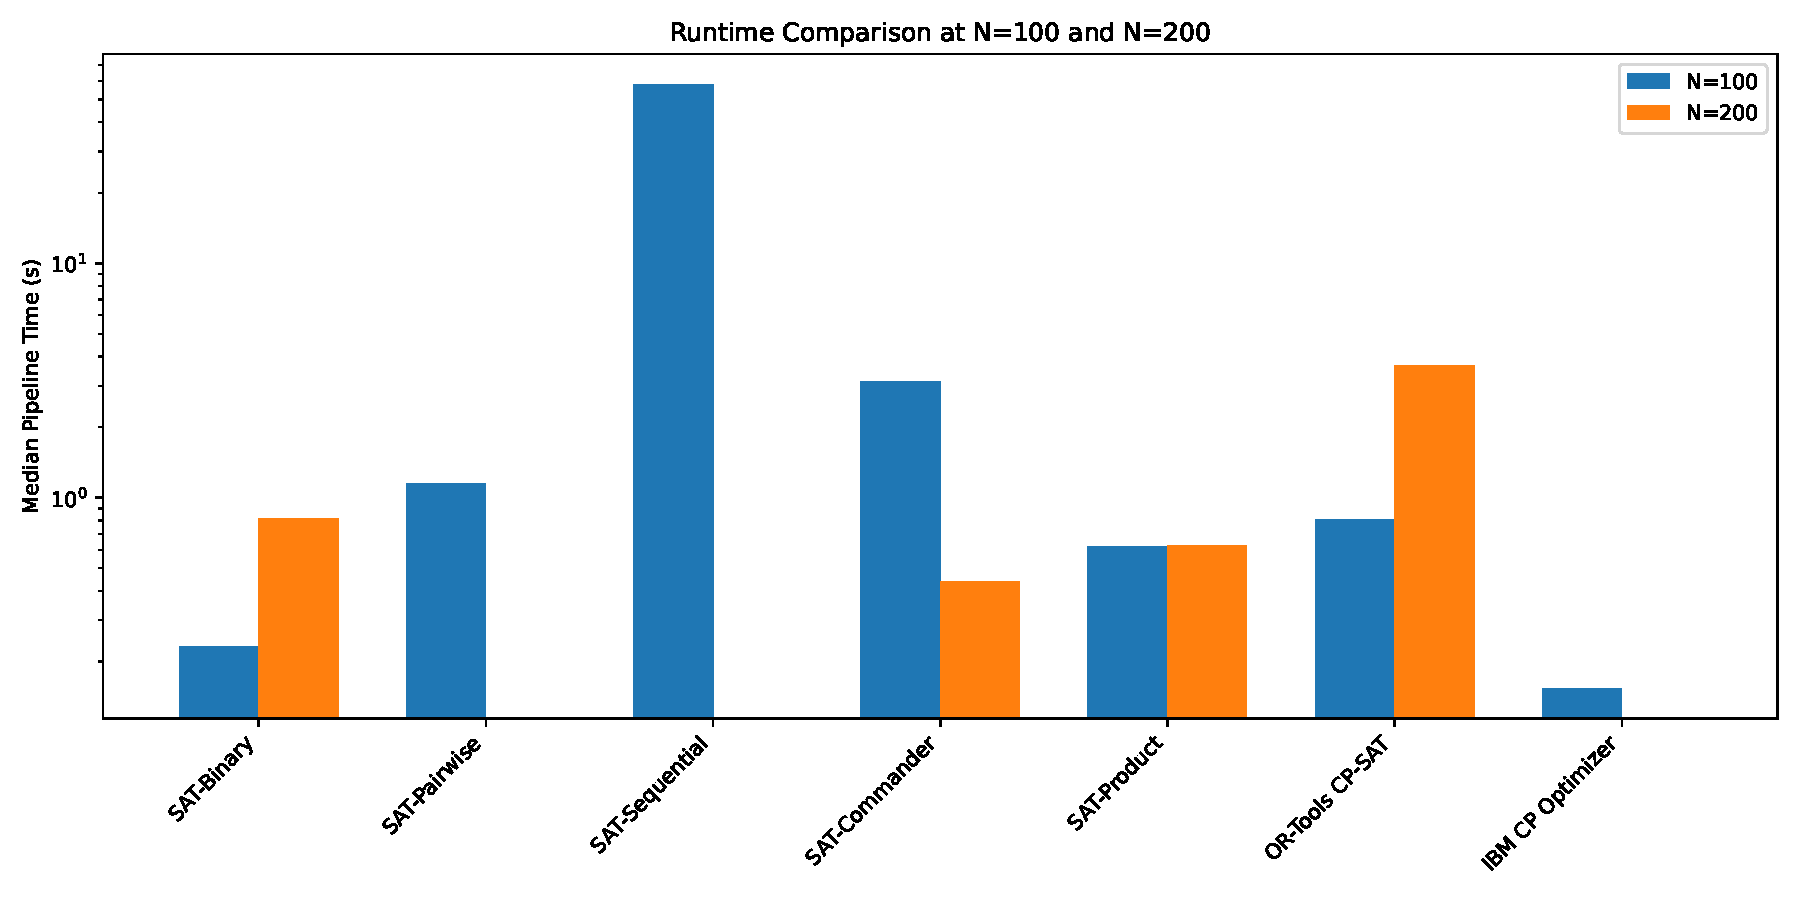
\includegraphics[width=0.8\textwidth]{../../results/figures/large_scale_n200/fig08_n100_vs_n200.pdf}
\caption{Median pipeline time comparison between $N=100$ and $N=200$ for successful methods.}
\label{fig:n100_vs_n200}
\end{figure}

As shown in Figure~\ref{fig:n100_vs_n200}, the methods that successfully scaled (SAT-Commander, SAT-Product, SAT-Binary, and OR-Tools CP-SAT) maintained manageable memory footprints due to their structural compactness. Interestingly, the SAT-Product encoding, which previously displayed non-monotonic failures and pathological timeouts at $N=44$ and $N=64$, effectively recovered at $N=200$ to achieve a median runtime of 0.627 seconds. Furthermore, SAT-Commander exhibited an inverted runtime scaling ratio (faster at $N=200$ than $N=100$), underscoring how specific variable partitioning strategies can favorably align with the default phase-saving heuristics of modern CDCL architectures on large symmetric grids.

\section{Conclusion}
\label{sec:conclusion}

This research provides a strictly controlled empirical evaluation of three major exact solving paradigms---Boolean SAT, Constraint Programming, and Mixed Integer Programming---on the N-Queens problem. Through the execution of 495 scheduled benchmark trials (430 successful completions) up to $N=100$, we observed that theoretical SAT structural compactness is a poor predictor of practical solving efficiency. Massive clause models (Pairwise) frequently outpaced compact-clause implementations (Sequential Counter). Under default heuristic settings, the SAT-Binary encoding emerged as the most efficient boolean model, completing $N=100$ in 0.231 seconds.

At $N=200$, the limitations of both hardware and software environments became evident. The SAT-Pairwise encoding was excluded due to an estimated memory footprint exceeding hardware limits, while IBM CP Optimizer encountered a license-imposed search space restriction. Among the successful methods at $N=200$, SAT-Commander achieved the fastest median resolution time of 0.441 seconds, significantly outpacing OR-Tools CP-SAT (3.672 seconds) and suggesting that optimal boolean partitioning can remain highly effective even at massive scales.
However, native Constraint Programming implementations handled the large state spaces efficiently. The IBM CP Optimizer recorded the fastest runtime overall, resolving $N=100$ in 0.153 seconds by circumventing the massive memory initialization bottlenecks required by SAT translation. Nevertheless, CP frameworks still suffer from exponential backtracks and do not universally eliminate search limitations. Furthermore, we documented severe non-monotonic search pathologies in the SAT-Product encoding, underscoring the extreme sensitivity of CDCL solvers to variable layout. 

Future investigations should focus on phase-policy ablation studies to isolate the mechanisms triggering SAT search pathologies, as well as evaluating these structural encodings on a broader suite of combinatorial benchmarks beyond placement constraints.


\bibliographystyle{cas-model2-names}
\bibliography{references}

\end{document}
